\section{Tutte's algorithm}

The basic graph theory terminology defined in the article ~\cite{pa, pb}
will be used.  Let $G=(V,E)$ be a planar graph. A mapping $\Gamma$ of $G$
into the plane is a function $\Gamma : V \cup E \to P(\mathbb{R}^2)$. This
function maps a vertex $v \in V$ to a point in $\mathbb{R}^2$ and an edge
$e = uv \in E$ to the straight line segment joining $\Gamma(u)$ and
$\Gamma(v)$.  A mapping is an embedding if distinct vertices are mapped to
distinct points and the open segment of each edge does not intersect any
other open segment of an edge or a vertex.
\\

A way to build embeddings of any planar, 3-connected graph $G=~(V,E)$ have
been produced by Tutte in 1963 ~\cite{pc}. Let $C$ be a cycle of
vertices. Those vertices are the vertices of a face of G in some (not
necessarily straight-line) embedding of $G$. Let $\Gamma$ be a mapping of
$G$ into the plane.

% In 1963, Tutte~\cite{pc} gave a way to build embeddings of any planar,
% 3-connected graph $G=~(V,E)$. Let $C$ be a cycle whose vertices are the
% vertices of a face of G in some (not necessarily straight-line) embedding
% of $G$. Let $\Gamma$ be a mapping of $G$ into the plane, satisfying the
% conditions:

% \begin{itemize}

% \item the set Ve of the vertices of the cycle C is mapped to the vertices of a strictly
% convex polygon Q, in such a way that the order of the points is respected;

% \item each vertex in $V_i = V \ V_e$ is a barycenter with positive coefficients of
% its adjacent vertices (Tutte assumed all coefficients to be equal to 1, but
% the proof extends without changes to this case). In other words, the images
% v of the vertices v under $\Gamma$ are obtained by solving a linear system
% (S): for each $u \in V_{i, v|uv \in E} \lambda_{uv} (u - v) = 0$, where the
% $\lambda_{uv}$ are positive reals. It can be shown that the system (S) admits
% a unique solution.

% \end{itemize}

\begin{theo} \label{theo:box} (Tutte’s Theorem) Let $Ve$ be a set of the
  vertices of the cycle $C$ mapped to the vertices of a strictly convex
  polygon $Q$, in such a way hat the order of the points is respected.  If
  for each vertex in $V_i = V \ V_e$ is a barycenter with positive
  coefficients of its adjacent vertices (Tutte assumed all coefficients to
  be equal to 1, but the proof extends without changes to this case), so
  $\Gamma$ is an embedding of $G$ into the plane, with strictly convex
  interior faces.
\end{theo}

\begin {figure}[H]
  \centering
  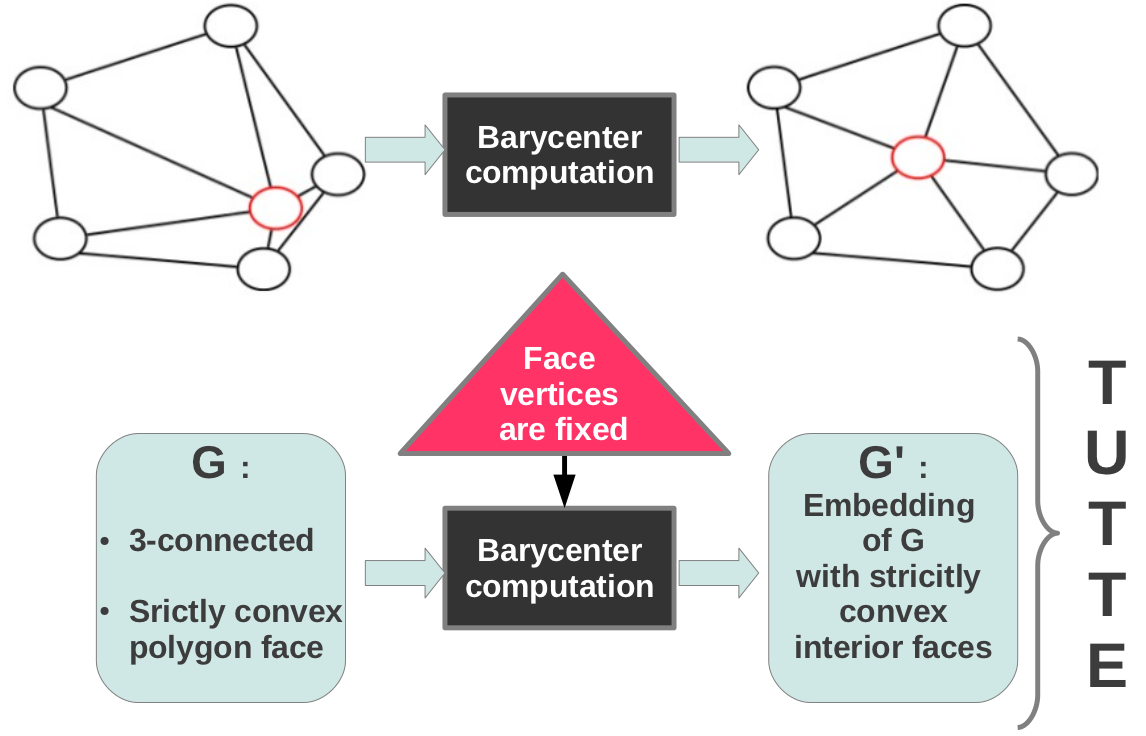
\includegraphics[scale=0.3]{img/tutte.png}
  \caption{Tutte's theorem illustration}
  \label{struct3}
\end {figure}

\subsection{Some extreme cases about Tutte's theorem}
In our project we do not use 3-connected graph but graph whose interior faces are triangle. It is obvious that considering the kind of graphs we used Tutte's theorem is verified because the fypothesis « All interior faces are tringle » is lighter than « 3-connected » hypothesis. So now we changed the hypothesis about the external polyhgon and the interior vertices in order to find out if the tutte's  is always verified.  

\subsubsection{Tutte's theorem and concave polygon}

In this section, we changed the hypothesis about the graph face. Now we consider a concave polygon face. Below is the illustration of a couterexample. 

\begin {figure}[H]
  \centering
  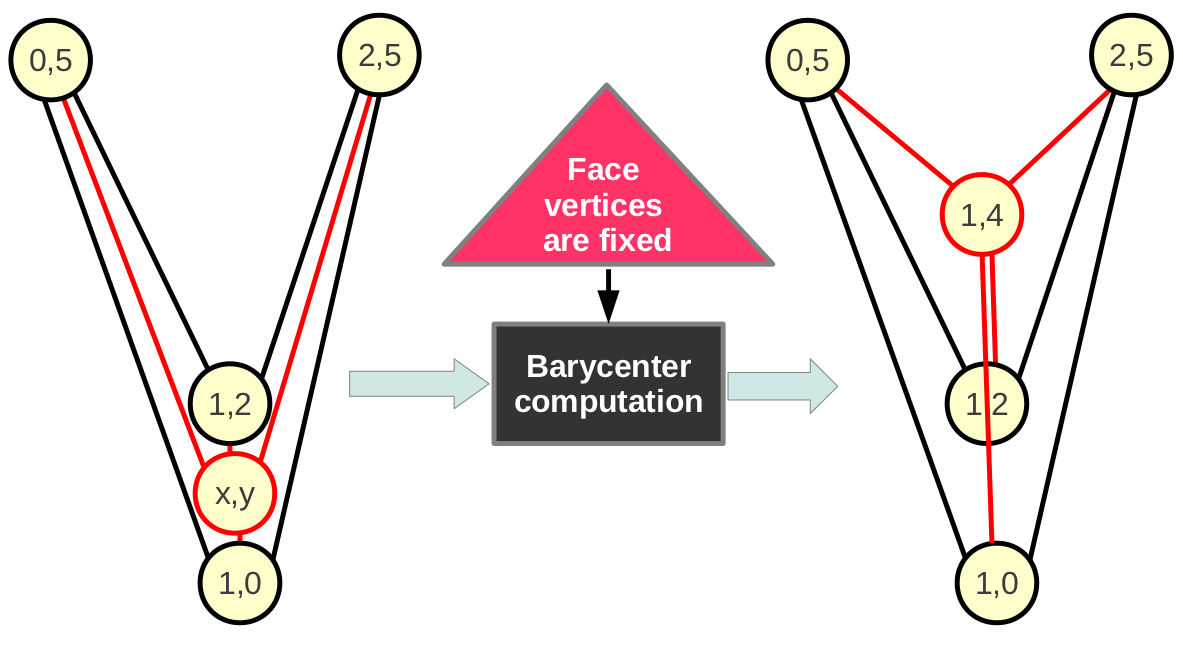
\includegraphics[scale=0.3]{img/tutte2.png}
  \caption{Tutte algorithm on concave polygon}
  \label{tutte2}
\end {figure}
\noindent
In the counterexample illustration above, the coordinate of the vertex shown in red color become $$(\frac{0+1+1+2}{4} , \frac{5+0+2+5}{4}) = (1 , 4)$$
One can see that after the the barycenter algorithm computation, the graph is no longer embedding. So the Tutte's theorem is not verified considering graphs with concave polygon face. 

\subsubsection{Tutte's algorithm and convex polygon with some fixed vertices}
This section kept the «convex polygon face» hypothesis but some internal vertices are considered fixed, their position never change during the barycenter algorithm computation. Below is the illustration of a couterexample. 

\begin {figure}[H]
  \centering
  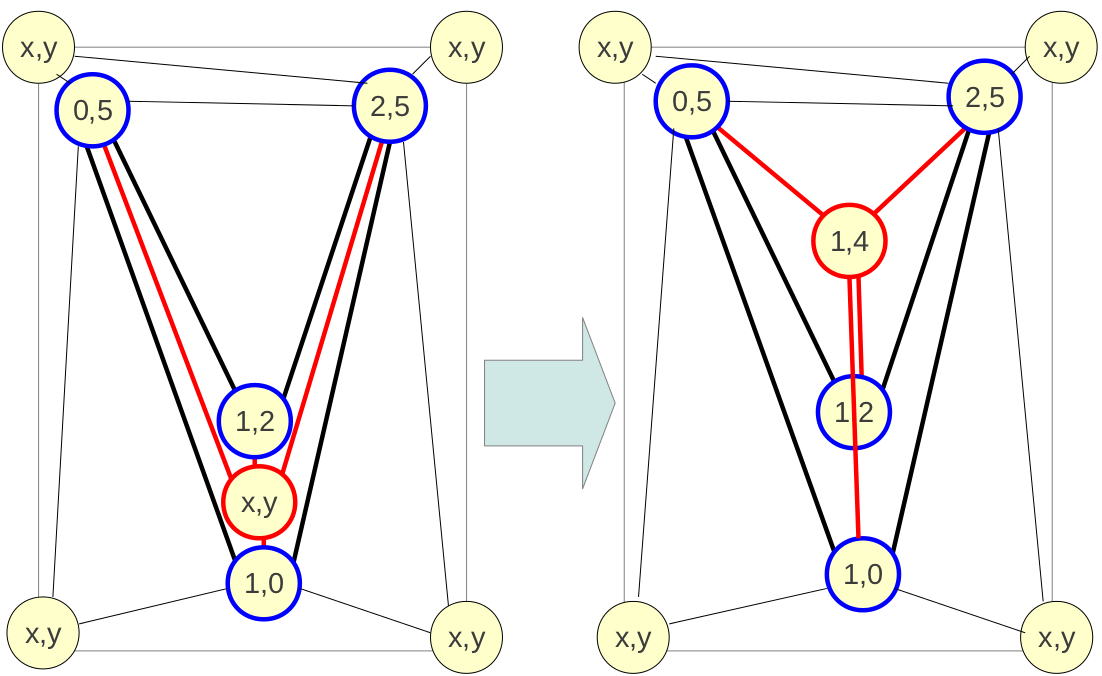
\includegraphics[scale=0.3]{img/tutte3.png}
  \caption{Tutte algorithm on convex polygon and fixes vertices}
  \label{tutte3}
\end {figure}
\noindent

As in the previous counterexample illustration (fig \ref{tutte2}) above, after the barycenter algorithm computation, the vertex shown in red color position changes. So the graph is no longer embedding which implies that the Tutte's theorem is not verified considering that some internal vertices can be fixed.


% \begin{thebibliography}{99}

% \bibitem{pa} E. Colin de Verdière, M. Pocchiola, and G. Vegter. Tutte's Barycenter Method applied to Isotopies. \emph{Computational Geometry: Theory and Applications, 26}, 81–97, 2003.

% \bibitem{pb} B. Bollob's. Modern graph theory, \emph{volume 184 of Graduate Texts in Mathematics}. Springer-Verlag, 1998.

% \bibitem{pc} W. T. Tutte. How to draw a graph. \emph{Proceedings of the London Mathematical Society}, 13:743–768, 1963.

% \end{thebibliography}


